\chapter{Parcourir une collection}
Un itérateur est une structure de donnés qui permet de parcourir une collection d'objets.
\exemple{
\texttt{\\
for(i=N-1 ; i >= 0 ; ++i);\\
}
Ici i joue le rôle d'un itérateur, il permet de parcourir une collection de N éléments du début à la fin ou de la fin au début.
}

Un itérateur est lié à une collection, on peut 
\begin{itemize}
	\item se placer en début/fin de la collection
	\item Passer à l'élément suivant/précédent de la collection
	\item savoir quand on est arrivé à la fin/début de la collection
\end{itemize}

En utilisant un langage pseudo objet, cela nous donnerai l'algorithme suivant : 
\begin{lstlisting}[numbers=none]
i = creerIterateur(c); //c étant la collection
for(i = debut(i); !videSuivant(i) ; i = suivant(i)) {
	//...
}
\end{lstlisting}

\begin{figure}[H]
\centering
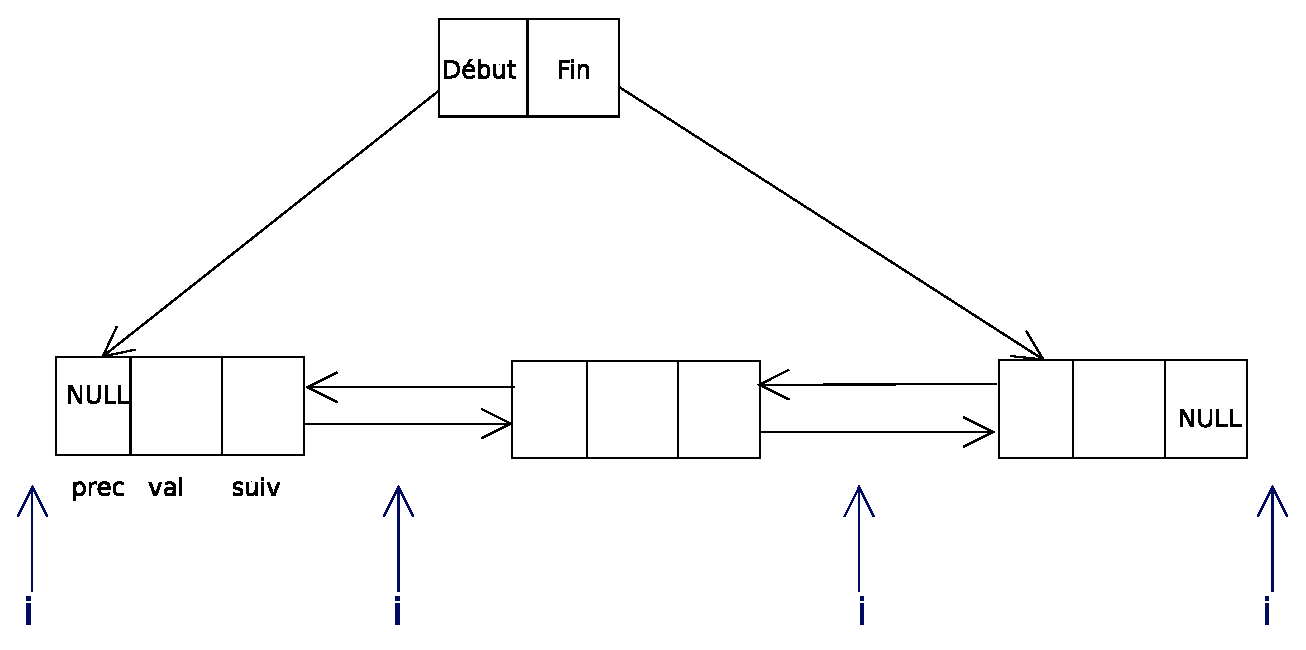
\includegraphics[width=15cm]{content/schemas/iterateur.eps}
\caption{Liste doublement chainée avec iterateur}
\end{figure}
\section{Itérateur sur la liste doublement chaînée}
Création d'un itérateur sur liste doublement chainée. % TODO cf
Écrire les fonctions suivantes:
\begin{description}
	\item[\texttt{creerIte}] Création d'un itérateur sur une \texttt{LDC} et place l'itérateur en début de liste
	\item[\texttt{next}] Déplace l'itérateur sur le suivant renvoie la valeur courant d'avant le déplacement 
	\item[\texttt{previous}] Déplace l'itérateur sur le précédent et renvoie la valeur d'avant le courant 
	\item[\texttt{hasNext}, \texttt{hasPrevious}] Renvoie 1 si l'élément suivant/précédent existe
	\item[\texttt{begin}, \texttt{end}] Plate l'itérateur sur le début/fin de la liste.
\end{description}

\lstinputlisting[language=C, caption=\texttt{Iterateur} sur \texttt{Liste} -- Header]{content/code/iterateur.h}
\lstinputlisting[language=C, caption=\texttt{Iterateur} sur \texttt{Liste} -- Implémentation]{content/code/iterateur.c}
